\documentclass[a4paper,10pt]{article}

\usepackage[utf8]{inputenc}
\usepackage[T1]{fontenc}
\usepackage[english]{babel}

\usepackage{color}
\usepackage{float}
\usepackage{caption}
\usepackage{subcaption}
\usepackage{fancyvrb}
\usepackage{tikz}
\usetikzlibrary{arrows, positioning, fit, backgrounds}

\usepackage{amssymb}
\usepackage{amsmath}
\usepackage{listings}
\usepackage{longtable}
\usepackage{graphicx}
\DeclareGraphicsExtensions{.png}

\title{DM529 -- Calculus\\ Exam
    \\ \rule{10cm}{0.5mm}}
\author{Sævar Berg Sævarsson \\ 111290 \\ Section S7 \\
\\Instructor: Magnus Gausdal Find\\ DM534\\\rule{5.5cm}{0.5mm}\\}
\date{\today}

\begin{document}
\maketitle
\vfill
\tableofcontents
\newpage
\section{Foo}
\label{sec:foo}
\begin{figure}[H]
\begin{center}
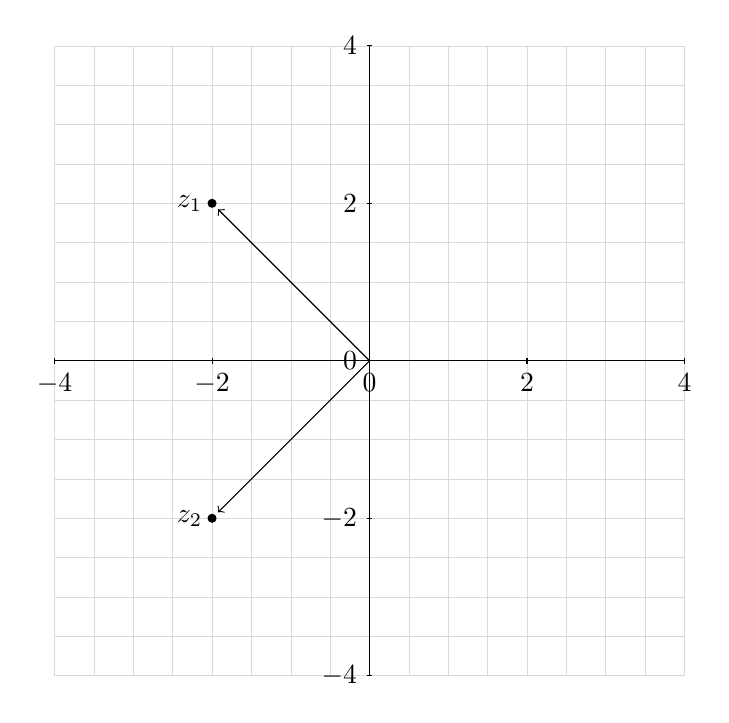
\begin{tikzpicture}[
    scale=1,
    point/.style=
        {inner sep=0pt,minimum size=1mm,draw,fill=black,circle}]
    \coordinate (p1) at (-2, 2);
    \coordinate (p2) at (-2, -2);
    \draw [step=0.5cm, gray!30, very thin] (-4,-4) grid (4,4);
    \draw (-4,0) -- (4,0);
    \draw (0, -4) -- (0, 4);
    \foreach \x in {-4,-2,...,4}
        \draw (\x cm,1pt) -- (\x cm,-1pt) node[anchor=north] {$\x$};
    \foreach \y in {-4,-2,...,4}
        \draw (1pt,\y cm) -- (-1pt,\y cm) node[anchor=east] {$\y$};
    \node [point] at (p1) {}
        edge [<-,shorten <=0.5mm] (0,0);
    \node [point] at (p2) {}
        edge [<-,shorten <=0.5mm] (0,0);
    \node at (p1) [anchor=east] {$z_1$};
    \node at (p2) [anchor=east] {$z_2$};
\end{tikzpicture}
\end{center}
\caption{Blah}
\label{fig:}
\end{figure}


\end{document}
